\section{GUI}

Allgemein wird von der GUI erwartet, dass die App intuitiv bedienbar ist und fehlerfrei auf möglichst vielen Hardware Typen dargestellt werden kann. \\

Des weiteren ist die GUI  Design so angelegt, dass die App jederzeit übersichtlich ein Maximum an Informationen darstellen kann.

\subsection{Startseite}
\label{subsec:Startseite}

Die Startseite der App soll dem User ermöglichen auf alle wichtigen Funktionen direkt zuzugreifen. Deshalb besteht diese nur aus folgenden vier Buttons {\color{IndianRed}\texttt{Neues Item}}, {\color{IndianRed}\texttt{Sammlung}}, {\color{IndianRed}\texttt{Leihwesen}} und {\color{IndianRed}\texttt{Info}}.

\begin{figure}[htbp]
	\centering
	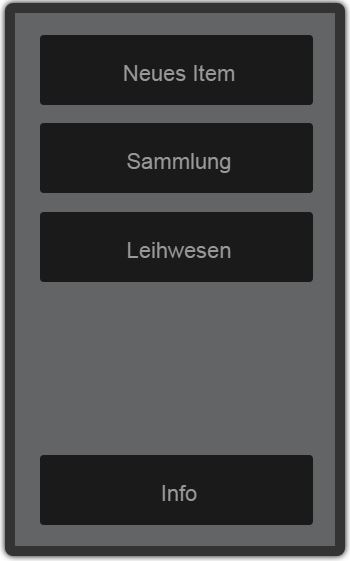
\includegraphics[scale=0.5]{pic/GUI/Main}
	\caption{Startseite}
\end{figure}

\subsection{Barcode Scannen}

Dieser Screen startet die eingebaute Kamera und wird automatisch angezeigt, wenn man ein neues Item anlegen will. Sollte das Item keinen Barcode besitzen, kann man von hier aus die Manuelle Eingabe erreichen. Eine zurück zur Startseite \ref{subsec:Startseite} ist ebenfalls möglich.

\begin{figure}[htbp]
	\centering
	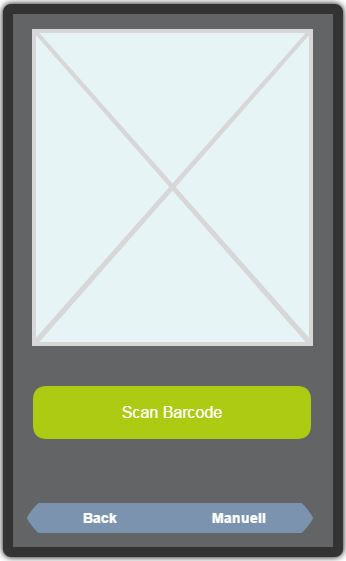
\includegraphics[scale=0.5]{pic/GUI/ScanBarcode}
	\caption{Barcode Scannen}
\end{figure}

\subsection{Manuell Anlegen / Item Bearbeiten}

Dieses Screenlayout wird sowohl für das manuelle Anlegen eines Items, als auch für das Bearbeiten eines vorhandenen Items genutzt.\\

Der einzige Unterschied besteht zwischen den beiden Aktionen darin, das dass beim manuellen Anlegen keine Datenelemente angezeigt werden. Während beim Bearbeiten eines Items, alle bisher gespeicherten Datenelemente angezeigt werden.

\begin{figure}[htbp]
	\centering
	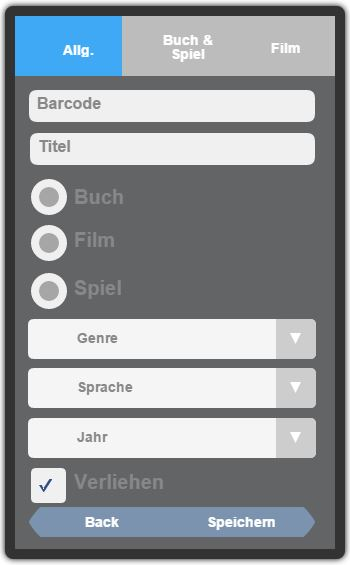
\includegraphics[scale=0.5]{pic/GUI/Manuell}
	\caption{Manuell Anlegen / Item Bearbeiten}
\end{figure}

\subsection{Detail Ansicht}

Hier werden dem User alle Datenelemente eines Items angezeigt. Ausserdem kann in dieser Ansicht das Item bearbeitet, verliehen oder gelöscht werden.

\begin{figure}[htbp]
	\centering
	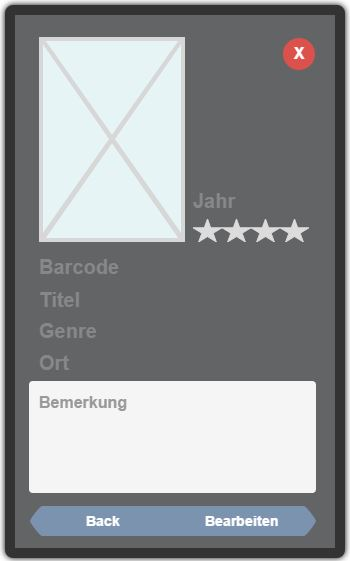
\includegraphics[scale=0.5]{pic/GUI/ItemAnsicht}
	\caption{Detail Ansicht}
\end{figure}

\subsection{Sicherheitsfrage Item Löschen}

Wenn der User ein Item aus der Datenbank (Sammlung) löschen will. Erscheint immer bevor der Löschvorgang gestartet wird folgende Sicherheitsfrage.

\begin{figure}[htbp]
	\centering
	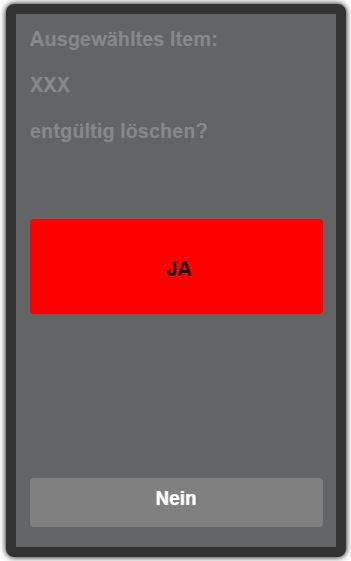
\includegraphics[scale=0.5]{pic/GUI/DeleteItem}
	\caption{Sicherheitsfrage}
	\end{figure}
	
\subsection{Item verleihen}

Wird ein Item als verliehen markiert, erscheint eine erweiterbare Liste mit Personen. Aus dieser Liste wählt der User nun die Person aus, welche das Item geliehen hat. Ist die Person noch nicht in der Liste, kann der User diese in die Liste eintragen.

\begin{figure}[htbp]
	\centering
	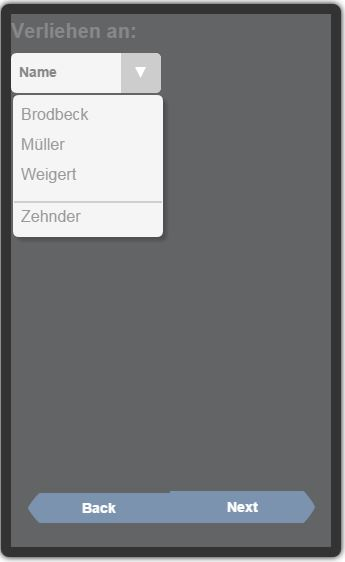
\includegraphics[scale=0.5]{pic/GUI/VerliehenAn}
	\caption{Item verleihen}
\end{figure}

\subsection{Filter}

Die Filteraktivität besteht aus einem Screen mit den drei Reitern {\color{IndianRed}\texttt{Allgemein}}, {\color{IndianRed}\texttt{Buch \& Spiel}} und {\color{IndianRed}\texttt{Film}}.

\subsubsection{Allgemein}

Folgende Datenelemente können auf dem Reiter {\color{IndianRed}\texttt{Allgemein}} \ref{fig:Allgemein} der Filter Activity gefiltert werden.\\

Barcode, Titel, Typ, Genre, Sprache, Erscheinungsjahr und Verliehen.

\begin{figure}[htbp]
	\centering
	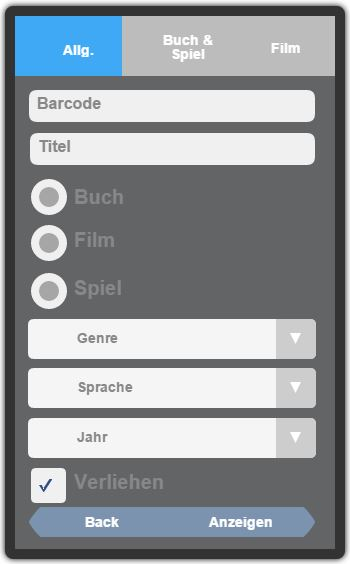
\includegraphics[scale=0.5]{pic/GUI/FilterAllgemein}
	\caption{Filter - Allgemein}
	\label{fig:Allgemein}
\end{figure}

\subsubsection{Buch \& Spiel}

Folgende Datenelemente können auf dem Reiter {\color{IndianRed}\texttt{Buch \& Spiel}} \ref{fig:BS} der Filter Activity gefiltert werden.\\

Für Bücher: Verlag, Autor und Auflage
Für Spiele: System und FSK

\begin{figure}[htbp]
	\centering
	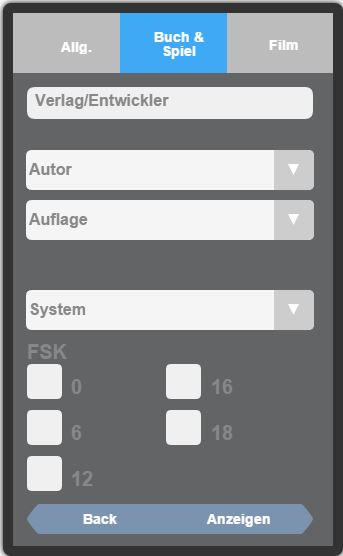
\includegraphics[scale=0.5]{pic/GUI/FilterBS}
	\caption{Filter - Buch \& Spiel}
	\label{fig:BS}
\end{figure}

\subsubsection{Film}

Folgende Datenelemente können auf dem Reiter {\color{IndianRed}\texttt{Film}} \ref{fig:Film} der Filter Activity gefiltert werden.\\

Studio, Regisseur, DVD, BlueRay und FSK

\begin{figure}[htbp]
	\centering
	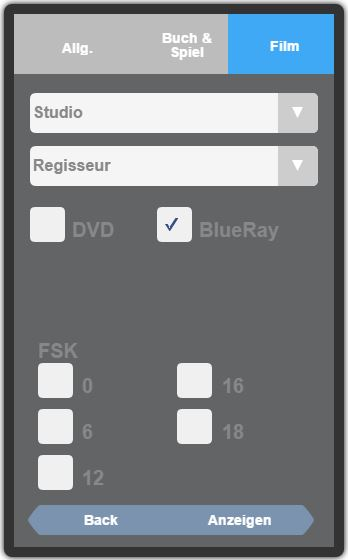
\includegraphics[scale=0.5]{pic/GUI/FilterFilm}
	\caption{Filter - Film}
	\label{fig:Film}
\end{figure}